% !TEX program = xelatex
% VERA-MOT implementation note; evidence current through 3 November 2026.
\documentclass[11pt,a4paper]{article}
\usepackage[a4paper,margin=24mm,headheight=15pt]{geometry}
\usepackage{fontspec}
\setmainfont{Liberation Serif}
\setsansfont{Liberation Sans}
\setmonofont{DejaVu Sans Mono}[Scale=0.77]
\usepackage{microtype}
\usepackage{amsmath,amssymb,mathtools}
\usepackage{booktabs,tabularx,array}
\usepackage{enumitem}
\usepackage{fancyhdr}
\usepackage{xcolor}
\usepackage{hyperref}
\usepackage{tikz}
\usetikzlibrary{arrows.meta,positioning,shapes.geometric}
\definecolor{paperblue}{HTML}{0F4669}
\definecolor{papermut}{HTML}{55606A}
\hypersetup{colorlinks=true,urlcolor=paperblue,citecolor=paperblue,linkcolor=paperblue,pdftitle={VERA-MOT: Reliability-Gated Appearance Association and Protected Feature Memory},pdfauthor={Charalampos Nadiotis}}
\newcommand{\codestr}[1]{\texttt{#1}}
\newcommand{\paperstatus}{\textsf{PRELIMINARY IMPLEMENTATION NOTE --- NOT PEER REVIEWED}}
\pagestyle{fancy}
\fancyhf{}
\fancyhead[L]{\footnotesize VERA-MOT / Implementation note / 2026-11-03}
\fancyhead[R]{\footnotesize Working draft v0.1}
\fancyfoot[C]{\thepage}
\renewcommand{\headrulewidth}{0.3pt}
\setlength{\parskip}{0.34em}
\setlength{\parindent}{0pt}
\setlist[itemize]{leftmargin=1.5em,itemsep=0.13em}
\setlist[enumerate]{leftmargin=1.6em,itemsep=0.14em}
\title{\vspace{-1em}\textbf{VERA-MOT: Reliability-Gated Appearance Association\\and Protected Feature Memory}\\\large A Reproducible Implementation Note for Multi-Object Tracking}
\author{Charalampos Nadiotis\\\normalsize Independent Robotics and Computer Vision Research\\\normalsize \href{https://github.com/n0711/vera-mot}{github.com/n0711/vera-mot}}
\date{3 November 2026 \quad | \quad Working draft v0.1}
\begin{document}
\maketitle
\vspace{-1.25em}
\begin{center}\fcolorbox{papermut}{white}{\parbox{0.87\linewidth}{\centering\small\textbf{\paperstatus}\\\vspace{2pt}Synthetic and code-level evidence only. No new real-vehicle tracking performance is claimed.}}\end{center}
\begin{abstract}
Visual re-identification (ReID) can support multi-object tracking when geometric association is ambiguous, but a poor-quality image crop can introduce misleading appearance evidence into both a matching decision and a track's persistent feature representation. This technical note specifies and implements a conservative, optional reliability gate for an existing pinned BoT-SORT association pipeline. The gate uses crop area, Laplacian-variance texture, and the fraction of a box inside the frame as observable image-quality proxies. Detections failing a fixed provisional threshold retain their geometric association path but do not participate in appearance matching or update the track's appearance memory. The implementation is provided as an explicitly opt-in patch and an independently testable project-owned module. On 3 November 2026, GitHub Actions reported 121 passing CPU tests and four passing pinned-tracker integration tests on synthetic inputs. These tests establish executable behaviour and specific memory invariants, \emph{not} improvements in vehicle identity accuracy, IDF1, HOTA, or identity-switch rate. We give a reproducibility record, mathematical definitions, limitations, and a prospective annotated-data evaluation protocol.
\end{abstract}
\textbf{Keywords:} multi-object tracking; appearance association; re-identification; image quality; feature memory; reproducibility.

\section{Introduction}
Tracking-by-detection assigns persistent identities to objects observed in successive frames. Motion, geometric overlap, and visual appearance can supply complementary association evidence. Methods such as Deep SORT and BoT-SORT incorporate an appearance representation into tracking \cite{wojke2017,aharon2022}, while ByteTrack highlights the importance of preserving useful low-confidence detections \cite{zhang2022}. These ideas do not imply that every extracted appearance vector is trustworthy.

For distant or blurred objects, an embedding may depend more on image artifacts than on discriminative object characteristics. Using such a vector may affect the immediate association and may also alter a running representation used for future matching. The project VERA-MOT (Visual Embedding Reliability Assessment for Multi-Object Tracking) studies whether a lightweight quality-based guard can reduce that risk. The present contribution is an implementation-level, falsifiable first slice, not a validated tracking improvement.

\textbf{Scope.} The code runs with the pinned BoT-SORT tracker and externally supplied frame-indexed detection boxes. It does not require recovering unavailable original training images, detector weights, or historic ReID checkpoints. It does not train a vehicle-specific embedding model, estimate true identity confidence, or validate field deployment. Existing archival benchmark summaries are kept distinct from new synthetic integration evidence.

\section{System Architecture and Contribution}
We separate image-derived appearance features from the decision about whether those features can influence track identity. The pipeline retains the underlying BoT-SORT geometric associations, the Kalman state, and its track lifecycle \cite{aharon2022}. The VERA policy only determines whether a new high-score detection contributes an appearance feature.

\begin{figure}[htbp]
\centering
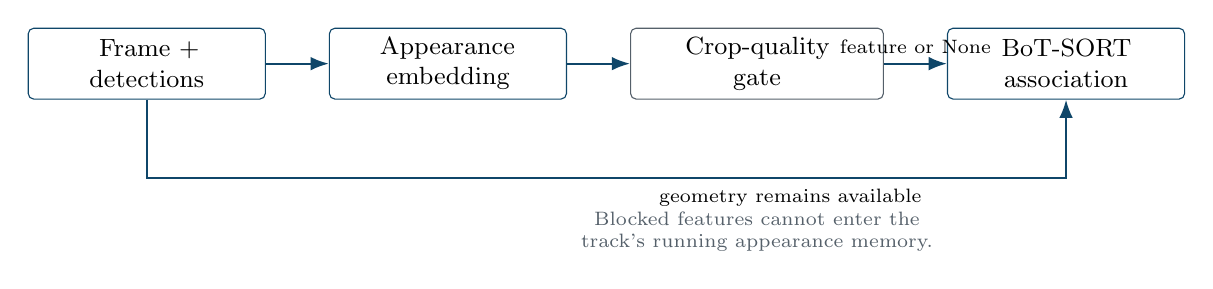
\begin{tikzpicture}[font=\small,>=Latex,node distance=8mm and 8mm,
 block/.style={draw=paperblue,rounded corners=2pt,align=center,minimum height=9mm,text width=28mm,inner sep=3pt},
 decision/.style={draw=papermut,rounded corners=2pt,align=center,minimum height=9mm,text width=30mm,inner sep=3pt},
 arr/.style={-Latex,thick,draw=paperblue}]
 \node[block] (det) {Frame +\\detections};
 \node[block,right=of det] (embed) {Appearance\\embedding};
 \node[decision,right=of embed] (gate) {Crop-quality\\gate};
 \node[block,right=of gate] (track) {BoT-SORT\\association};
 \draw[arr] (det) -- (embed);
 \draw[arr] (embed) -- (gate);
 \draw[arr] (gate) -- node[above,font=\scriptsize]{feature or None} (track);
 \draw[arr] (det.south) -- ++(0,-10mm) -| node[below,pos=0.35,font=\scriptsize]{geometry remains available} (track.south);
 \node[below=13mm of gate,align=center,font=\scriptsize,text=papermut] {Blocked features cannot enter the\\track's running appearance memory.};
\end{tikzpicture}
\caption{Proposed implementation path. The gate is executed \emph{after} embeddings are extracted; this version makes no claim of computational savings.}
\label{fig:architecture}
\end{figure}

The implemented changes are: (i) a deterministic, fail-closed crop-quality module, (ii) a narrow opt-in compatibility patch that conveys missing appearance features to the pinned tracker's existing association logic, (iii) a protected-memory invariant, and (iv) dataset-free CPU and real-upstream synthetic integration tests. The implementation lives in project-owned source and traceable patches rather than an unrecorded mutation of third-party tracking code.

\section{Reliability Proxy}
Let detection $j$ at time $t$ have a proposed image-space bounding box $B_{tj}=(x_1,y_1,x_2,y_2)$ and a valid clipped region $\widetilde B_{tj}$ inside the frame. Let $A_{tj}$ and $\widetilde A_{tj}$ denote their areas, respectively. The following bounded cues are computed:
\begin{align}
q_{\mathrm{size}}(t,j) &= \operatorname{clip}\!\left(\frac{\widetilde A_{tj}}{A_0},0,1\right), \qquad A_0=1024\;\mathrm{px}^2, \\[-1pt]
q_{\mathrm{focus}}(t,j) &= \operatorname{clip}\!\left(\frac{\operatorname{Var}(\nabla^2 I_{tj}^{\mathrm{gray}})}{L_0},0,1\right), \qquad L_0=120, \\
q_{\mathrm{frame}}(t,j) &= \operatorname{clip}\!\left(\frac{\widetilde A_{tj}}{A_{tj}},0,1\right), \\
q(t,j) &= \min\{q_{\mathrm{size}},q_{\mathrm{focus}},q_{\mathrm{frame}}\}, \\
g(t,j) &= \mathbf{1}[q(t,j)\ge \tau], \qquad \tau=0.5.
\label{eq:quality}
\end{align}
Here $\operatorname{clip}(z,0,1)=\min(1,\max(0,z))$, $I_{tj}^{\mathrm{gray}}$ is the image crop converted to grayscale, and $\nabla^2$ denotes the discrete Laplacian used by OpenCV. Invalid coordinates or arrays fail validation rather than producing an implicit high-quality feature. An image region smaller than $2\!\times\!2$ pixels receives a zero focus score.

\textbf{Interpretation.} $q_{\mathrm{frame}}$ measures boundary truncation only; it cannot detect occlusion by a foreground object. The focus proxy measures high-frequency content, not certainty of correct identity. A uniformly coloured but correctly observed vehicle may score poorly. The reference area, variance and threshold are provisional, with no empirical calibration against vehicle identity labels.

\section{Association and Memory Invariant}
The original BoT-SORT appearance-enabled path evaluates an embedding distance and geometric distance and combines them under spatial-proximity restrictions. Our interface keeps these equations in the upstream tracker, but changes how missing appearance evidence is represented. For a new detection, let $f_{tj}$ be the normalized extracted vector. The feature handed to the tracking stage is
\begin{equation}
\widehat f_{tj}=\begin{cases}
f_{tj}, & g(t,j)=1,\\
\varnothing, & g(t,j)=0.
\end{cases}
\label{eq:masked-feature}
\end{equation}
For track $i$ with stored smooth feature $s_i$, the adapted embedding-distance function is
\begin{equation}
d_{\mathrm{app}}(i,j)=\begin{cases}
1-\dfrac{s_i^\top\widehat f_{tj}}{\lVert s_i\rVert\lVert\widehat f_{tj}\rVert}, & s_i,\widehat f_{tj}\ne\varnothing,\\[5pt]
2, & \text{otherwise.}
\end{cases}
\label{eq:distance}
\end{equation}
In the pinned tracker, the appearance distance is divided by two and distances above the appearance threshold are rejected. Thus the missing-feature sentinel $2/2=1$ excludes that appearance pair but preserves the existing IoU/motion route. The sentinel is an interface convention, \emph{not} a measured cosine distance.

Suppose track $i$ has smooth appearance memory $s_i^{t-1}$. If the new matched detection is gated off, the desired invariant is
\begin{equation}
g(t,j)=0\ \land\ j\mapsto i\ \Longrightarrow\ s_i^t=s_i^{t-1}.
\label{eq:invariant}
\end{equation}
The implementation achieves this by constructing the new track observation with no appearance feature. The pinned STrack update path only calls its feature-history update when a current feature is present. A later accepted observation may resume appearance updates. Matching can still fail geometrically; the invariant does not guarantee recovered identity.

\section{Implementation and Reproducibility}
The project pins BoT-SORT to revision \codestr{251985436d6712aaf682aaaf5f71edb4987224bd}. The M4.5 bridge injects a project-owned feature encoder while deferring an unnecessary upstream FastReID import. An opt-in M4.6 patch adds the gate hook and handles the $\varnothing$ appearance case. Local installers check source revision and known content fingerprints and refuse unrelated source edits; the submodule pointer is not moved.

The user-facing runner accepts video frames plus a CSV containing \codestr{frame,x1,y1,x2,y2,score}, uses either a baseline colour-histogram embedder or a separately supplied generic image encoder, and outputs MOT-format association hypotheses with JSON provenance. The M4.6 mode is explicitly named \codestr{vera-hsv-reid}; the baseline \codestr{hsv-reid} remains selectable. The histogram is not a trained vehicle ReID model. Neither mode consumes the original unavailable model checkpoints.

The integration depends on the following tracked source and tests:
\begin{itemize}
\item \codestr{src/vera\_mot/reid\_reliability.py}: crop-quality gate and counters.
\item \codestr{src/vera\_mot/botsort\_reid\_bridge.py}: checked tracker and policy attachment.
\item \codestr{patches/botsort-vera-quality-gate.patch}: optional upstream hook and missing-feature handling.
\item \codestr{tests/test\_vera\_reid\_quality\_gate.py}: proxy and memory-invariant regression checks.
\item \codestr{tests/test\_vera\_reid\_video\_integration.py}: paired real-upstream processing of generated video.
\end{itemize}
The complete procedure and constraints are documented in \href{https://github.com/n0711/vera-mot/blob/main/docs/VERA_REID_RELIABILITY.md}{the repository protocol}. The versioned release checkpoint is the repository's main-branch M4.6 merge on 3 November 2026. This manuscript is a documentation artifact; publication of source code is not independent scientific replication.

\section{Verified Test Evidence}
\begin{table}[htbp]
\centering\small
\caption{Observed GitHub Actions results for the M4.6 implementation, 3 November 2026. Checks are synthetic or code-level, not annotated vehicle tracking benchmarks.}
\begin{tabularx}{\linewidth}{@{}p{0.37\linewidth}X@{}}
\toprule
\textbf{Check or artifact} & \textbf{Observed evidence and its interpretation} \\
\midrule
CPU suite & 121 tests passed; 5 integration-marked tests deselected. Unit tests do not establish field accuracy. \\
Pinned BoT-SORT runtime smoke & 4 integration tests passed; 16 non-integration tests deselected. These exercise generated data, missing-feature matching and protected memory. \\
Patch applicability and idempotence & Pinned-source compatibility check passed; repeat installation of the opt-in gate patch passed. \\
Generated synthetic sequence & Eight frames and 14 supplied detections in the rectangle demonstration; a functioning interface test, not an identity-labelled video study. \\
Historical no-ReID dataset summary & Repository reports HOTA $43.340$, IDF1 $56.964$, and $1{,}180$ ID switches for its frozen 20-sequence baseline. Original inputs and weights are unavailable here; the values were not recomputed in this milestone. \\
New annotated vehicle experiment & \textbf{Not performed.} No comparative VERA HOTA, AssA, IDF1, switch-rate or latency measurements exist. \\
\bottomrule
\end{tabularx}
\label{tab:evidence}
\end{table}

Passing a synthetic memory test verifies a property of the implementation under that controlled input. It does not imply that quality gating decreases identity switches under real occlusion, scale change, moving cameras or compression. In particular, the historical no-ReID summary cannot be used as a denominator for an unrun gated-versus-ungated comparison.

\section{Evaluation Protocol for a Future Study}
A scientifically meaningful comparative study should lock the detector outputs, frame sequence, camera-motion compensation, track thresholds and identity annotations before selecting an appearance policy. The predeclared conditions should include (1) no ReID; (2) ungated appearance; and (3) quality-gated appearance with identical embeddings. The gate's parameters should be selected from training/validation identities only, with a separate held-out evaluation.

The primary association outcomes should include IDF1 and association accuracy (AssA), supplemented by HOTA, identity-switch counts, identity fragmentation and re-identification accuracy after specified temporal gaps \cite{luiten2021}. Quality-gate false rejections should be measured using annotated visibility/quality where available. Repeated runs should record per-sequence metrics, input checksums, configuration hashes, runtime versions and the source revision. GPU or CPU latency must be profiled separately, especially because the current quality evaluation follows feature extraction and cannot yet save extraction time.

\section{Limitations and Threats to Validity}
\begin{enumerate}
\item \textbf{Domain mismatch.} Synthetic coloured rectangles do not reproduce true vehicle appearance, scale, perspective or occlusion.
\item \textbf{Uncalibrated quality.} Laplacian variance conflates focus and texture; boundary clipping is not an occlusion label.
\item \textbf{Appearance model.} HSV histograms and generic pretrained image features are not vehicle-specific ReID models. No new model training or retrieval benchmark was performed.
\item \textbf{No causal performance evidence.} The implementation tests establish code paths and invariants but no improvement in MOT accuracy, inference latency or robustness.
\item \textbf{Limited reproducibility of prior results.} The historical detector and dataset artifacts are not distributed with the source; their prior aggregate metrics are archival rather than newly independently validated.
\item \textbf{Policy granularity.} A Boolean hard gate can discard valid fine-grained appearance cues; a calibrated continuous model may be preferable, but that is a separate research hypothesis.
\end{enumerate}

\section{Conclusion}
The M4.6 VERA-MOT implementation makes a narrow mechanism testable: new low-quality appearance observations may be blocked from appearance matching and track-feature memory without deleting the ordinary geometric association path. A pinned-tracker integration and synthetic regression evidence support implementation correctness within their stated scope. Whether the mechanism improves identity continuity for real vehicles remains an \emph{open empirical question}. The next publishable evaluation milestone is a controlled, identity-annotated vehicle experiment comparing ungated and gated conditions with fixed inputs, parameters and provenance.

\section*{Reproducibility and Status Statement}
Working technical note, 3 November 2026. Source: \url{https://github.com/n0711/vera-mot}. The public source release is not an assertion of peer review. This note does not present new measured UAVDT outcomes or re-identification accuracy on real vehicles. Any future amended manuscript must record new evidence and version changes instead of silently replacing these limitations.

\begin{thebibliography}{9}
\bibitem{wojke2017} N. Wojke, A. Bewley, and D. Paulus, ``Simple Online and Realtime Tracking with a Deep Association Metric,'' \emph{IEEE International Conference on Image Processing}, 2017. doi: \href{https://doi.org/10.1109/ICIP.2017.8296962}{10.1109/ICIP.2017.8296962}.
\bibitem{aharon2022} N. Aharon, R. Orfaig, and B.-Z. Bobrovsky, ``BoT-SORT: Robust Associations Multi-Pedestrian Tracking,'' arXiv:2206.14651, 2022. \url{https://arxiv.org/abs/2206.14651}.
\bibitem{zhang2022} Y. Zhang, P. Sun, Y. Jiang, et al., ``ByteTrack: Multi-Object Tracking by Associating Every Detection Box,'' \emph{European Conference on Computer Vision}, 2022. doi: \href{https://doi.org/10.1007/978-3-031-20047-2_1}{10.1007/978-3-031-20047-2\_1}.
\bibitem{luiten2021} J. Luiten, A. O\v{s}ep, P. Dendorfer, et al., ``HOTA: A Higher Order Metric for Evaluating Multi-Object Tracking,'' \emph{International Journal of Computer Vision}, vol. 129, pp. 548--578, 2021. doi: \href{https://doi.org/10.1007/s11263-020-01375-2}{10.1007/s11263-020-01375-2}.
\end{thebibliography}
\end{document}
